\chapter{Neural Networks and Machine Translation}
\pagestyle{fancy}\lhead{\textbf \footnotesize\it{Neural Networks and Machine Translation}}
\pagestyle{fancy}\chead{} \pagestyle{fancy}\rhead{}
\pagestyle{fancy}\lfoot{\textbf {\small\it{Univ-Mascara/Computer Science: 2024}}} 
\pagestyle{fancy}\cfoot{} \pagestyle{fancy}\rfoot{\thepage}
%%%%%%%%%%%%%%%%%%%%%%%%%%%%%%%%%%%%%%%%
\section{Overview}\label{start3}
In this chapter, we embark on an in-depth exploration of neural networks, pivotal to understanding the intricate workings of machine translation. 
Beginning with a thorough examination of the foundational feed-forward networks (FFNs), recurrent neural networks (RNNs), long short-term memory networks (LSTMs), and gated recurrent units (GRUs), we lay the groundwork for comprehending the neural machine translation (NMT) process. 

We delve into the nuances of training NMT models, and the decoding phase, where trained models generate translations from input sequences. 
Finally, we conducted a comprehensive survey of recent advancements and methodologies in neural machine translation research, with a focus on exploring related works specifically dedicated to the Arabic language context.

\section{Neural Networks}
Neural networks are the foundational computational mechanisms driving Neural Machine Translation, employing complex algorithms to mimic human language understanding and generation. 
At the core of these networks is the node, or processing unit, which functions similarly to neurons in the human brain. 
Each node is designed to receive inputs—typically a vector of real-valued numbers—process these inputs through a series of mathematical operations, including weighted sums and activation functions, and then produce an output that can be passed on to subsequent layers or nodes in the network.
The following subsections will delve into the different types of neural networks, beginning with the simplest form: the feed-forward neural network.

\subsection{Feed-Forward Neural Networks}
A feed-forward neural network is a basic type of neural network where information moves in one direction from the input to the output layer without any loops or cycles back to previous layers. 
Outputs from each node are forwarded upwards to the subsequent layer without any feedback to lower levels. 
An illustration, referred to as Figure~\ref{fig:ffn}, shows a FFN consisting of two layers. 
These networks are composed of three distinct types of nodes: input, hidden, and output. 
The input nodes receive individual scalar values, and notably, among these input nodes is a constant bias node, labeled $x_0$, which is always set to the value of 1. 
In the hidden layer, nodes calculate a weighted sum of their inputs and then apply a nonlinear function to this sum to determine their output.
\begin{figure}[h]
	\centerline{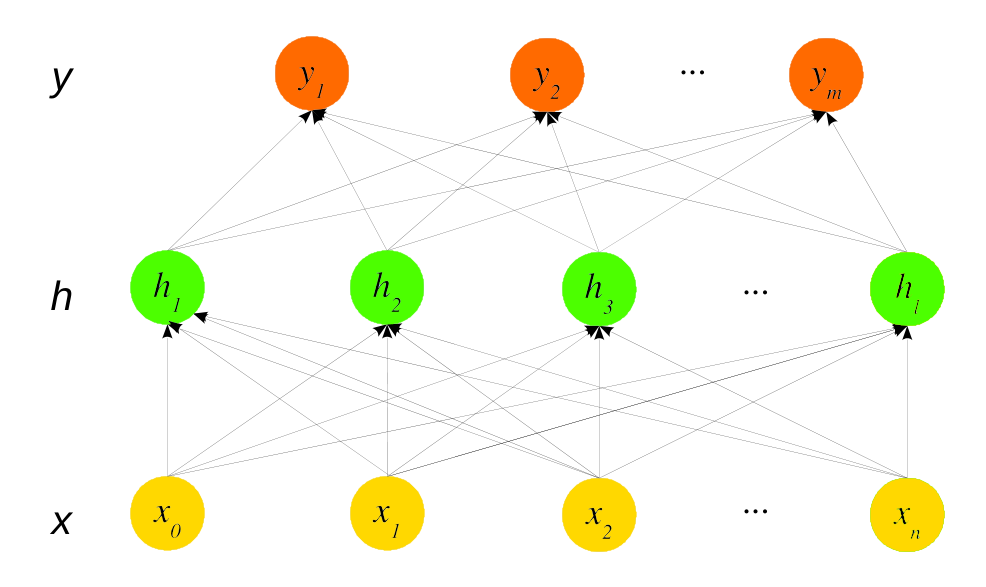
\includegraphics[width=0.7\linewidth]{Figures/FFN}}
	\caption{A feed-forward network consisting of two layers includes an input layer $x$, a hidden layer $h$, and an output layer $y$.}
	\label{fig:ffn}
\end{figure}
In a standard neural network structure, every layer is comprehensively interconnected, allowing nodes to receive inputs from all nodes in the preceding layer. 
These networks are characterized by their depth, with numerous layers contributing to their complexity. 
Hidden nodes within these layers act as automatic feature detectors, eliminating the need for manual feature identification by learning to recognize relevant patterns in the input data through training. 
Each hidden node is defined by its parameters, including a weight vector and a bias term. 
The parameters for the entire hidden layer are aggregated into a weight matrix $U$, where each weight $u_{jk}$ in $U$ corresponds to the connection strength from the $k^{th}$ input node $x_k$ to the $j^{th}$ hidden node $h_j$, and a bias vector that applies to the entire layer.

A notable feature of neural networks is the incorporation of non-linear activation functions, with the rectified linear unit ($ReLU$) standing out for its simplicity and widespread usage. 
$ReLU$ is particularly efficient to compute, as depicted in Figure~\ref{fig:relu} (a). 
This function returns the value of $z$ when $z$ is greater than 0 and returns $0$ when $z$ is less or equal to 0.
\begin{figure}[h]
	\centering
	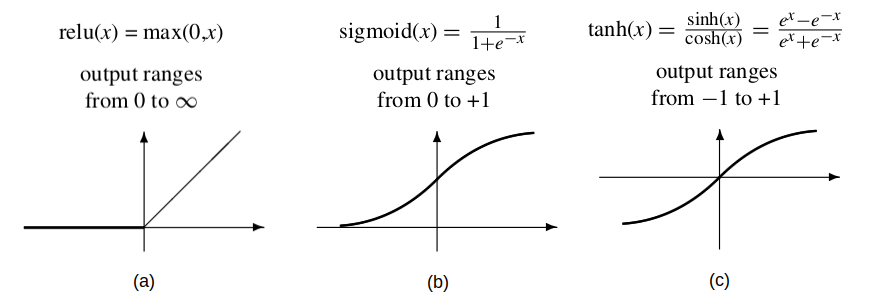
\includegraphics[width=0.7\linewidth]{Figures/Relu}
	\caption{Common activation functions utilized in neural networks.}
	\label{fig:relu}
\end{figure}
The $sigmoid$ (or logistic) function, another frequently utilized activation function, has been illustrated in Figure~\ref{fig:relu} (b).
An activation function similar to the sigmoid but more widely employed is the hyperbolic tangent ($tanh$), depicted in Figure~\ref{fig:relu} (c).

The computation of the hidden layer in the basic feed-forward network can be performed efficiently using straightforward matrix operations, involving three main steps:
\begin{itemize}
	\item The multiplication of the weight matrix by the input vector $x$,
	\item Addition of the bias vector, and
	\item Application of the activation function $f$, such as $ReLU$, $sigmoid$, or $tanh$.
\end{itemize}
Hence, the neural network depicted in Figure~\ref{fig:ffn} can be expressed mathematically as follows: 
\begin{itemize}
	\item A set of input nodes represented by the vector $x = (x_1, x_2, x_3, . . . , x_n)^T$;
	\item A set of hidden nodes represented by the vector $h = (h_1, h_2, h_3, . . . , h_l)^T$;
	\item A set of output nodes represented by the vector $y = (y_1, y_2, y_3, . . . , y_m)^T$;
	\item A weight matrix connecting input nodes to hidden nodes denoted by $U = u_{jk}$;
	\item A weight matrix connecting hidden nodes to output nodes denoted by $W = w_{ij}$.
\end{itemize}
The computation of the hidden layer output, represented by the vector $h$, is performed according to Equation~\ref{eqn:hj}, incorporating the activation function $f$.
\begin{equation}
	h_j = f(\sum_{k}u_{jk}x_k)
	\label{eqn:hj}
\end{equation}
The value $h$ obtained serves as a representation of the input. 
Subsequently, the output layer's function is to utilize this revised representation $h$ and calculate a conclusive output, as described in Equation~\ref{eqn:yi}.
\begin{equation}
	y_i = \sum_{j}w_{ij}h_j
	\label{eqn:yi}
\end{equation}
In numerous instances, this output may initially be a real-valued number; however, it is often transformed into a probability distribution using a $softmax$ function. For a vector $y$ with a dimensionality of $d$, the $softmax$ function is defined as shown in Equation~\ref{eqn:softmax_yi}, where $1 \leq i \leq d$.
\begin{equation}
	softmax(y_i) =\frac{e^{y_i}}{\sum_{j}e^{y_j}}
	\label{eqn:softmax_yi}
\end{equation}
The $softmax$ function operates on a vector $y = [y_1, y_2, y_3, . . . , y_m]$ of arbitrary values, transforming them into a probability distribution where each value falls within the range of (0, 1) and the sum of all values equals one.

\subsection{Recurrent Neural Networks}
A neural network containing a cycle inside its network connections is called a recurrent neural network (RNN). 
Its preceding outputs directly or indirectly influence the value of a node. 
Figure~\ref{fig:rnn} illustrates the structure of a simple RNN based on \cite{elman90}. 
Similar to conventional FFNs, the values for a layer of hidden nodes are calculated by multiplying an input vector representing the current input, $x$, by a weight matrix and then passing the result through a non-linear activation function. 
The associated output, $y$, is then determined using the hidden layer, which comprises the hidden nodes. 
The context layer is where it differs from a FFN the most. 
It keeps the previous values and sends them to the appropriate nodes in the hidden layer. 
This layer uses the hidden layer’s value from the previous time step as input to the computation at the hidden layer.
\begin{figure}[h]
	\centering
	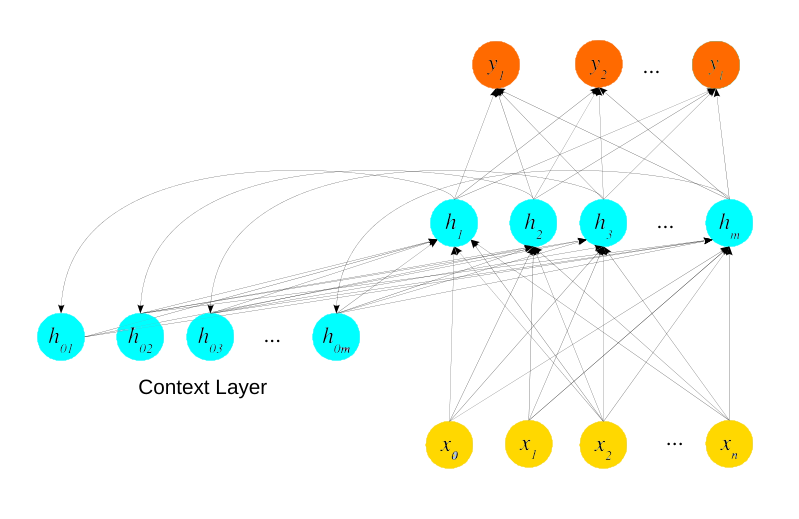
\includegraphics[width=0.7\linewidth]{Figures/RNN}
	\caption{A basic recurrent neural network.}
	\label{fig:rnn}
\end{figure}

\subsubsection{Stacked Recurrent Neural Networks} 
Stacked recurrent neural networks (RNNs) consist of multiple layers, where the output of one layer serves as the input to the next layer. 
Information flows from lower layers to higher layers, and the final output is generated by the top layer. 
Stacked RNNs have shown improved performance in neural MT compared to single-layer networks \cite{bahdanau15}. 
This improvement can be attributed to the network's ability to create representations at different levels of abstraction across the layers. 
However, the optimal number of stacked RNNs depends on the availability of training data. 
While abundant data can lead to better generalization, limited data may result in overfitting \cite{lample18}. 
Moreover, increasing the number of stacked layers escalates the training costs.

\subsubsection{Bidirectional Recurrent Neural Networks}
In recurrent networks, the hidden state at any given time encapsulates all information about the sequence up to that point, serving as the left context for the current input. 
In neural machine translation (NMT), having access to the entire input sequence simultaneously suggests the importance of utilizing the context to the right of the input. 
Training an RNN in reverse on the input sequence is one approach to retain this information. 
Combining the forward and backward networks results in a bidirectional RNN, where two independent RNNs process input from start to finish and finish to start, respectively \cite{schuster97}. 
The outputs of both networks are then merged to create a unified representation incorporating both left and right input contexts at each time step. 
Methods such as concatenation, element-wise operations, or averaging can be employed to combine the outputs of the forward and backward passes. 
This ensures that the information on both sides of the current input is captured in the output at each time step.
Figure~\ref{fig:rnn-brnn} illustrates the conventional RNN structure alongside the BRNN architecture over a timeline. In the RNN, only a forward hidden layer is present, whereas in the BRNN, both forward and backward hidden layers are depicted.

\begin{figure}[h]
	\centering
	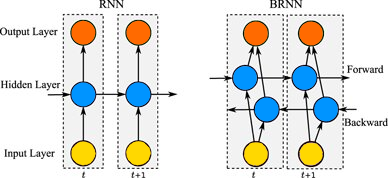
\includegraphics[width=0.9\linewidth]{Figures/RNN-BRNN}
	\caption{Architecture of RNN and BRNN shown over a period of time.}
	\label{fig:rnn-brnn}
\end{figure}

\subsection{Long Short-Term Memory}
One of the main limitations of RNNs in machine translation is their difficulty in handling long-distance dependencies. Distant words play a crucial role in translation tasks, as demonstrated in the following example:
\begin{quotation}
	The lengthy \textit{sentence} composed of numerous words spanning multiple lines still \textit{poses} significant challenges for MT.
\end{quotation}
In this example, the verb \textit{poses} depends on the subject \textit{sentence}, which is separated by a long subordinate clause.

While RNNs can access preceding sequences, the knowledge retained in hidden states tends to be relatively localized. 
Consequently, more complex network structures have been developed to address the difficulty of maintaining context over extended periods. 
It is essential for the network to discard irrelevant information while retaining data crucial for future decision-making. 
Long Short-Term Memory (LSTM) and Gated Recurrent Units (GRUs) are the predominant approaches employed to achieve this objective.

LSTM networks, introduced by \cite{hochreiter97}, address the challenge of managing context by dividing it into two sub-problems: removing unnecessary information and incorporating data crucial for future decisions. 
Unlike incorporating a fixed strategy into the architecture, the key lies in learning to handle context dynamically. 
LSTMs accomplish this by expanding the architecture with an explicit context layer and employing specialized neural units with gates to control the flow of information within the network layers. 
These gates utilize additional weights to sequentially process input, previous hidden layers, and previous context layers.

\subsection{Gated Recurrent Units}
GRU, akin to LSTM but with fewer parameters, offers the advantage of reduced training costs by requiring fewer parameters. 
This reduction in parameters is achieved by eliminating the need for a separate context vector and reducing the number of gates, thereby alleviating the computational burden compared to LSTM. 
Both GRU and LSTM employ sigmoid functions in their gates to either allow information with values close to one to pass through or block information with values close to zero. 

In contrast to simple FFNs, LSTMs and GRUs feature more complex neural nodes, as depicted in Figure~\ref{fig:lstm-vs-gru}, with inputs and outputs connected to each node type. 
The additional complexity within LSTM and GRU nodes is primarily contained within the nodes themselves. 
The only external complexity introduced by LSTM, beyond the basic recurrent node, is the availability of the other context vector as an input and output. 
Conversely, GRU nodes exhibit similar input and output architecture to the simple recurrent node.
\begin{figure}[h]
	\centering
	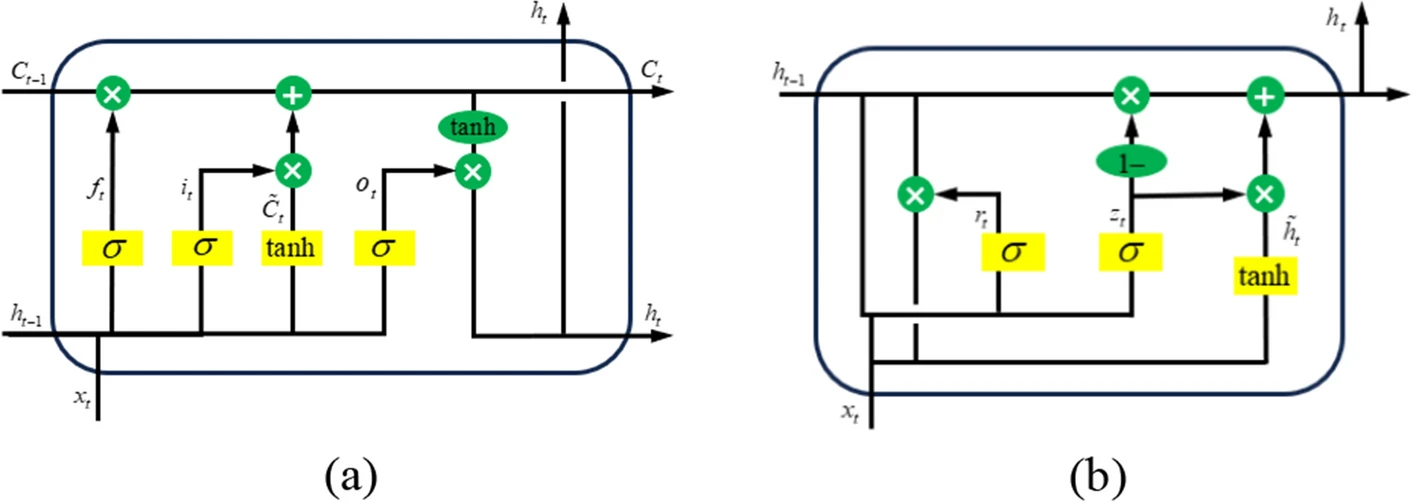
\includegraphics[width=0.7\linewidth]{Figures/LSTM-vs-GRU}
	\caption{Diagram illustrating the network structure of LSTM in the first panel (a) and GRU in the second panel (b)}
	\label{fig:lstm-vs-gru}
\end{figure}

\section{Neural Machine Translation}
The standard architecture for Neural Machine Translation (NMT) is the encoder-decoder network. 
This architecture operates on the fundamental principle of employing an encoder network to convert a sequence of words from the source language sentence into a contextual representation. 
Subsequently, a decoder utilizes this representation to generate an output sequence, essentially providing a plausible translation into the target language. 
Figure~\ref{fig:encoder-decoder} illustrates the encoder-decoder architecture at its most abstract level, comprising three key components: an encoder, context, and decoder. 
The encoder takes in a source language sentence as an input sequence of words, $x_1, x_2, ..., x_m$, and produces a corresponding sequence of contextualized representations known as a context vector. 
This context vector captures the essence of the input and serves as input to the decoder. 
Finally, the decoder utilizes the context vector to generate the most probable translation as a sequence of words, $y_1, y_2, ..., y_n$. 
Encoders and decoders can be implemented using either RNNs or Transformers.
\begin{figure}[h]
	\centering
	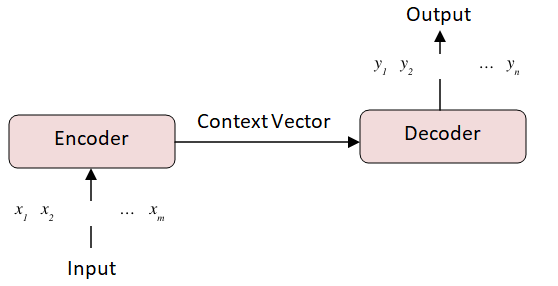
\includegraphics[width=0.7\linewidth]{Figures/Encoder-Decoder}
	\caption{Basic Encoder-Decoder architecture}
	\label{fig:encoder-decoder}
\end{figure}

Figure 2.7 illustrates a simplified version of the RNN-based encoder-decoder architecture. 
The encoder processes the input sequence $x$ with the objective of generating a representation of the input. 
This representation is captured in the final hidden state of the encoder, represented as $h^e_n$. 
Subsequently, this context representation, denoted as $c$, is transferred to the decoder. 
Upon receiving this state, the decoder utilizes it to initialize its initial hidden state. 
The first decoder cell employs $c$ as its initial hidden state, $h^d_0$, and proceeds to generate a sequence of outputs iteratively, one element at a time, until an end-of-word marker, </s>, is produced. 
Consequently, each hidden state is dependent on the preceding hidden state and the output generated in the preceding state. 
The embedding layer is composed of word embeddings, which adhere to the notion that semantically related words in similar contexts should possess similar representations. 
Ultimately, the output $y$ at each time step involves a $softmax$ computation over the vocabulary, $V$. The most probable output at each time step can be determined by computing the $argmax$ over the $softmax$ output as per Equation~\ref{eqn:yt}. 
Although Figure~\ref{fig:rnn-encoder-decoder} illustrates a single network layer, stacked and bi-directional networks are typically employed for both the encoder and decoder in practical implementations.
\begin{equation}
	\hat{y}_t = argmax_{w \in V}P(w|x, y_1, . . . , y_{t-1})
	\label{eqn:yt}
\end{equation}
\begin{figure}[]
	\centering
	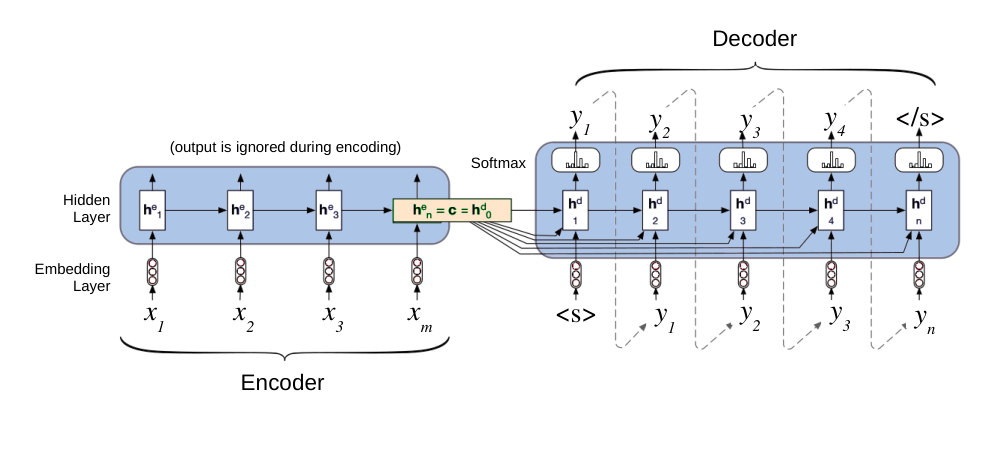
\includegraphics[width=1.0\linewidth]{Figures/RNN-Encoder-Decoder}
	\caption{The basic RNN-based encoder-decoder architecture.}
	\label{fig:rnn-encoder-decoder}
\end{figure}

A significant drawback of this architecture lies in its inability to evenly represent information from the beginning of a sentence, particularly evident in lengthy sentences. 
To address this issue, the attention mechanism emerges as a solution. 
It enables the decoder to access information from all the hidden states of the encoder, rather than solely relying on the last hidden state. 
The concept behind the attention mechanism is to create a singular context vector, denoted as $c$, by computing a weighted sum of all the encoder's hidden states. 
These weights concentrate on a specific segment of the source text pertinent to the token generated by the decoder. 
Notably, the context vector produced by the attention mechanism is dynamic, varying for each decoded token. 
By introducing the attention mechanism, the static context vector is replaced with $c_i$ a dynamically derived counterpart from the encoder's hidden states at each decoding step $i$, ensuring comprehensive consideration of all encoder states.

\subsection{Training Neural Machine Translation Models}
Neural Machine Translation (NMT) operates within a supervised machine learning framework, where the correct output, denoted as $y$, is known for each input observation, $x$. 
The system's output, represented as $\hat{y}$, serves as an estimate of the actual $y$. 
During the training phase, the objective is to adjust the parameters within each layer so that $\hat{y}$ closely resembles $y$ for every training instance.
To accomplish this, a loss function is employed to quantify the disparity between the system's output and the actual output. 
The optimization process, typically facilitated by the gradient descent algorithm, seeks to minimize this loss function by adjusting the parameters. 
Gradient descent utilizes the gradient of the loss function, computed as the partial derivative of the loss function with respect to each parameter, to iteratively update the model's parameters. 
However, in the realm of neural networks, characterized by numerous layers and millions of parameters, computing the partial derivative of a weight in one layer concerning the loss associated with another layer necessitates employing techniques such as error back-propagation or reverse differentiation. 
These methodologies are crucial for efficiently navigating the complex landscape of neural network optimization.

Moreover, NMT models undergo end-to-end training, where each training instance comprises a pair of sentences, one in the source language and the other in the target language. These sentence pairs are concatenated with a designated separator token, <s>, to form the training data. Typically, this training data is sourced from established datasets containing aligned pairs of sentences, known as parallel corpora. Optimization within the NMT framework is characterized by a non-convex problem landscape.
Nevertheless, there exist several best practices for effectively training NMT models. For instance, it is advisable to initialize the model weights with small random numbers and to employ random seeds for reproducibility. Additionally, normalizing the input values to have zero mean and unit variance can be beneficial in enhancing training stability and convergence.

NMT model training involves multiple epochs, representing complete iterations over the training data. Typically, as training progresses, the error on the training set steadily decreases. However, a key challenge arises when the model starts to overfit, meaning it memorizes the training data excessively without generalizing well to unseen examples. To diagnose overfitting, a separate set of examples known as the development (or validation) set is used, which is not involved in the training process. Monitoring the error on this development set over the course of training reveals a point where the error begins to increase, indicating overfitting.
In theory, training should halt when the minimum error on the development set is reached. However, in practice, this is more nuanced for NMT models due to the non-deterministic nature of training and the lack of clear convergence or overfitting points, particularly with sizable datasets. While some studies suggest stopping criteria based on approximate training durations or a fixed number of epochs, most NMT research does not specify precise stopping conditions. To mitigate overfitting, various regularization techniques are employed, such as dropout, which randomly disables some nodes and connections during training.

In addition to regularization, hyperparameter tuning plays a crucial role in NMT architecture design. These hyperparameters, which include the learning rate, mini-batch size, number of layers, hidden nodes per layer, and activation functions, are chosen by the architect to optimize model performance.
\subsection{Decoding}
The decoding (inference) algorithm employed to generate translations (as illustrated in the Figure~\ref{fig:rnn-encoder-decoder}) faces a challenge. 
Opting for the single most probable word at each step implies a 1-best greedy search, where a greedy algorithm makes locally optimal decisions. 
However, there are instances where following a sequence of words leads to the realization that an earlier mistake was made. 
In such cases, the best sequence may initially comprise less probable words that are refined by subsequent words in the context of the entire output. 
For instance, when translating an idiomatic expression, the initial words chosen may seem unusual (e.g., "\textit{take your hat off}" for "\textit{respect, admire, or congratulate someone}").

In NMT decoding, the predominant method employed is known as beam search. 
Unlike selecting the best word at each step, beam search maintains $k$ possible words, where $k$ denotes the beam size or beam width. 
Initially, a $softmax$ is computed over the entire vocabulary to assign probabilities to each word. 
From this $softmax$ output, the k-best candidates are selected, forming hypotheses. 
Each hypothesis represents an initial output sequence along with its probability. 
These top $k$ hypotheses are progressively expanded by passing them through different decoders in subsequent steps. 
At each decoder, a $softmax$ is generated over the entire vocabulary to determine the next word for each hypothesis. 
Subsequently, each of the $k * V$ potential sequences is scored based on the product of the current word's probability and the path leading to it. 
These hypotheses are then pruned down to the $k$ best ones to ensure there are never more than $k$ hypotheses at any given time. 
This iterative process continues until a complete translation candidate marked by "</s>" is generated, signifying the end of a hypothesis. 
The finished hypothesis is then removed, and the beam size is reduced by one. 
This search persists until the beam size diminishes to zero, resulting in $k$ hypotheses. 
The best translation is determined from the complete hypothesis with the highest score. 
Figure~\ref{fig:beam} illustrates this process using a beam size of six.
When evaluating the top paths, we assess each based on the product of their word prediction probabilities. 
In practical applications, we tend to achieve improved outcomes by normalizing the score according to the length of the translation produced, which involves dividing the score by the number of words. 
This normalization process occurs after the search is finalized.
\begin{figure}
	\centering
	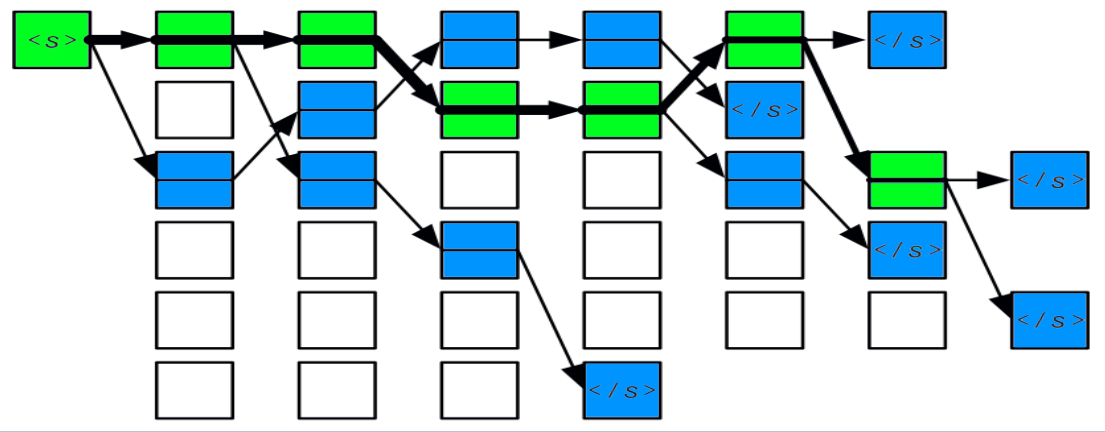
\includegraphics[width=0.7\linewidth]{Figures/beam}
	\caption{Beam search decoding with a beam size of six.}
	\label{fig:beam}
\end{figure}

\section{Related Work}
In the recent years, Research in AMT has predominantly centered on Neural MT, targeting translation from Arabic to English and various other languages. 
Neural machine translation, in particular, has become a compelling substitute for phrase-based Statistical Machine Translation (SMT), especially for the Arabic language.
Numerous studies are currently focusing on the translation between Dialectal Arabic and Modern Standard Arabic (MSA) in low-resource settings, both from Dialectal Arabic to MSA and vice versa.
Table~\ref{tab_ANMT} summarizes the surveyed Neural-based AMT research studies.
\begin{small}
	\begin{longtable}{|l|l|l|l|l|}
		\caption{Neural-based AMT researches}
		\label{tab_ANMT}\\
		\hline
		Year & Research & SL-TL$^{\mathrm{a}}$ & Method & Score\\
		\hline
		\endhead
		%	\hline
		%	\endfoot
		
%		\multicolumn{5}{c}{\textbf{Corpus-based AMT researches}}\\
		%	\hline
		\multicolumn{5}{l}{\textbf{Neural-based AMT}}\\
		\hline
		2016 & Almahairi et al. \cite{almahairi16}		& Ar$\leftrightarrow$En &MT Evaluation& 49.7/33.62\\
		2016 & Guzm{\'a}n et al. \cite{guzman16}		& En$\rightarrow$Ar &Morpho-syntactic analysis& +75\%\\
		2017 & Belinkov et al. \cite{belinkov17}		& Ar$\leftrightarrow$En &Morpho/Vocab/Factored NMT&Bl 28.42\\
		2017 & Durrani et al. \cite{durrani17}			& Ar$\leftrightarrow$En &MT Evaluation& Bl +4\\	
		2017 & Choi et al. \cite{choi17}				& Kor$\rightarrow$Ar &Corpus extension&Bl 27.07\\
		2018 & Almansor \& Al-Ani \cite{almansor18}		& Ar$\rightarrow$En &Low-resource& Bl +10\\
		2018 & Shapiro \& Duh \cite{shapiro18}			& Ar$\rightarrow$En &Morpho/Vocab/Factored NMT&Bl 29.10\\
		2018 & Alrajeh \cite{alrajeh18}					& Ar$\rightarrow$En &MT Evaluation& Bl +13\\
		2018 & Alkhatib \& Shaalan \cite{alkhatib18}	& Ar$\leftrightarrow$En &Paraphrasing model& 86.9\%/94.1\%\\
		2018 & Baniata et al. \cite{baniata18}			& DA$\rightarrow$MSA &Multitask Learning& 0.41/0.30\\
		2019 & Aqlan et al. \cite{aqlan19}				& Ar$\rightarrow$Cn &Pre-/Post-processing& Bl 24.66\\
		2019 & Oudah et al. \cite{oudah19}				& Ar$\rightarrow$En &Pre-/Post-processing& 55.64/53.54\\
		2019 & Hadj Ameur et al. \cite{hadjameur19}		& Ar$\leftrightarrow$En &Pre-/Post-processing&29.76/20.41\\	
		2019 & Gashaw \& Shashirekha \cite{gashaw19}	& Amh$\rightarrow$Ar &MT Evaluation& Bl 12\\	
		2020 & Ji et al. \cite{ji20}					& $\rightarrow$Ar &Multilingual/Low-resource& 25.49\\
		2021 & Bensalah et al. \cite{bensalah21}		&  Ar$\rightarrow$En &Pre-processing/MT Evaluation& 41.87\%\\
		2021 & Berrichi \& Mazroui \cite{berrichi21}	& Ar$\leftrightarrow$En & Morpho/Vocab/Factored NMT&Bl 33.02\\	
		2021 & Moukafih et al. \cite{moukafih21}		& DA$\leftrightarrow$Ar &Multi-Task learning/MT Eval&Bl 35.06\\	
		2021 & Nagoudi et al. \cite{nagoudi21}			& DA$\rightarrow$En &Pre-processing/MT Evaluation& Bl 25.72\\	
		2021 & Stergiadis et al. \cite{stergiadis21}	& Ar$\rightarrow$En &Multidimensional Tagging&Bl 50.84\\	
		2022 & Bensalah et al. \cite{bensalah22}		& Ar$\rightarrow$En &MT Evaluation&Bl 0.575\\	
		2022 & Slim et al. \cite{slim22}				& DA$\rightarrow$MSA &Transductive transfer learning&Bl 35.87\\
		2022 & Gaser et al. \cite{gaser22}				& DA$\rightarrow$En &Segmentation& chrF2 51.3\\
		2022 & Nagoudi et al. \cite{nagoudi22}			& 20 lang$\rightarrow$Ar &Multi-lingual model& Bl 32.07\\
		2022 & Hameed et al. \cite{hameed22}			& Ru$\rightarrow$Ar & MT Evaluation& 51.57\% \\
		2022 & Baniata et al. \cite{baniata22}			& DA$\rightarrow$Ar & RPE$^{\mathrm{b}}$+sub-word & Bl 66.87\\
\hline
\multicolumn{3}{l}{$^{\mathrm{a}}$Source language-Target language}&
\multicolumn{2}{l}{$^{\mathrm{b}}$Reverse Positional Encoding}\\
\end{longtable}
\end{small}

\section{Summary}
In this chapter, we embarked on a comprehensive exploration of neural networks, particularly focusing on feedforward networks (FFN), recurrent neural networks (RNN), long short-term memory networks (LSTM), and gated recurrent units (GRU). 
These architectures lay the foundation for understanding the mechanisms behind neural machine translation (NMT). 

We delved into the intricacies of training NMT modelsand the decoding phase, where the trained models generate translations from input sequences. 
Finally, we delved into related works in the field, dedicating special attention to advancements, methodologies, and challenges specific to neural machine translation in the context of the Arabic language.